\section{Sistemi Embedded}\label{sistemi-embedded}

Sistemi (a microcontrollore) di elaborazione atti a svolgere una
specifica funzione o compito (special-purpose), non ri-programmabili e
incorporati in un sistema complesso.

Le loro caratteristiche principali:

\begin{itemize}
\item
  \textbf{Funzionalità specifica}: eseguono sempre le stesse cose
  ripetutamente;
\item
  \textbf{Tightly constrained ed efficienza}: memoria e CPU limitate;
\item
  \textbf{Uso di design metrics}: dimensioni, performance e consumo di
  energie;
\item
  \textbf{Progettati per essere efficient}i: efficienza energetica, di
  code-size, di run-time, di peso e di costo;
\item
  \textbf{Affidabilità};
\item
  \textbf{Reattivi e/o real time}: permettono di avere un tempo di
  risposta basso o quasi nullo.
\end{itemize}

\subsection{CPS - Cyber Physical
System}\label{cps---cyber-physical-system}

Sono un'integrazione di diversa natura con lo scopo di controllare un
processo fisico e il suo adattamento in tempo reale attraverso feedback.

\subsection{Architettura sistema
embedded}\label{architettura-sistema-embedded}

Non c'è ne una di riferimento, ma esistono molteplici piattaforme, una
struttura di base potrebbe essere:

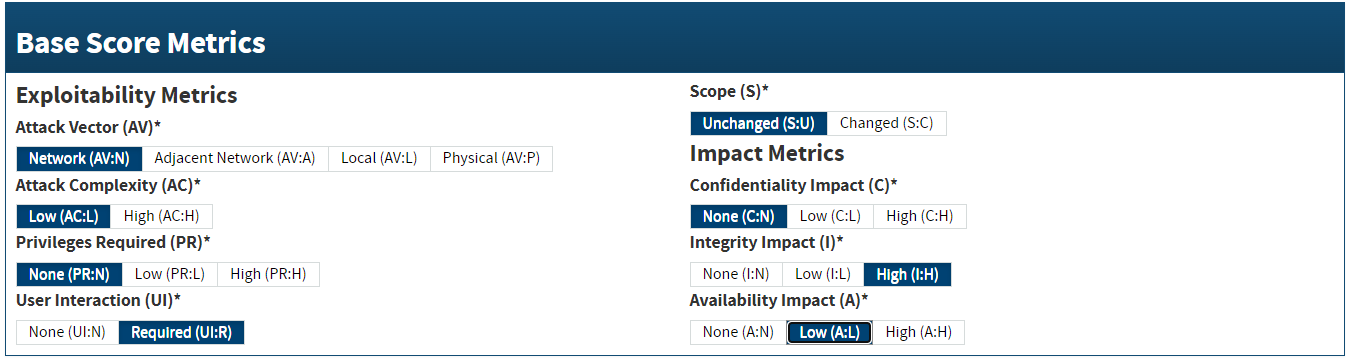
\includegraphics[width=6.26772in,height=2.69444in]{media/image26.png}

\subsubsection{CPU}\label{cpu}

Possono essere 3:

\begin{itemize}
\item
  \textbf{General-purpose}:architettura e insieme di istruzioni
  predefinito, comportamento definito dal programma in esecuzione;
\item
  \textbf{Application-specific processor (ASIP)}: programmabili e
  ottimizzati per classi di applicazioni;
\item
  \textbf{Single-purpose}: progettati per implementare una specifica
  funzionalità o programma.
\end{itemize}

Ma quale scegliere fra un processore \textbf{GPP} (general purpose) o
\textbf{ASP} (application specific)?

I primi sono CPU di base che tramite l'utilizzo delle architetture di
Von Neumann e Harvard permettono l'uso di software personalizzato per
una specifica applicazione.

I secondi sono sistemi che danno soluzioni a specifiche applicazioni con
un numero limitato di funzioni che non giustificano architetture più
complesse.

\subsubsection{MCU}\label{mcu}

Dispositivo integrato su un singolo circuito elettronico, evoluzione al
microprocessore ed utilizzato nei sistemi embedded.

Composto da un processore, una memoria permanente e volatile, canali di
I/O, gestore interrupt e blocchi specializzati.

Alcuni esempi possono essere gli Arduino dove si programma esternamente
e si passa il file già buildato pronto all'esecuzione.

\subsubsection{SOC e Single-Board PC}\label{soc-e-single-board-pc}

Sta per System on a chip, un unico chip incorpora un sistema completo.

\section{Microcontrollori}\label{microcontrollori}

Programmabile tramite sistema esterno, viene creato e buildato il file
poi passato al microcontrollore con USB o seriale.

I microcontrollori non hanno S.O. quindi tutto ciò passato viene
eseguito dal processore.

\subsection{Elementi base}\label{elementi-base}

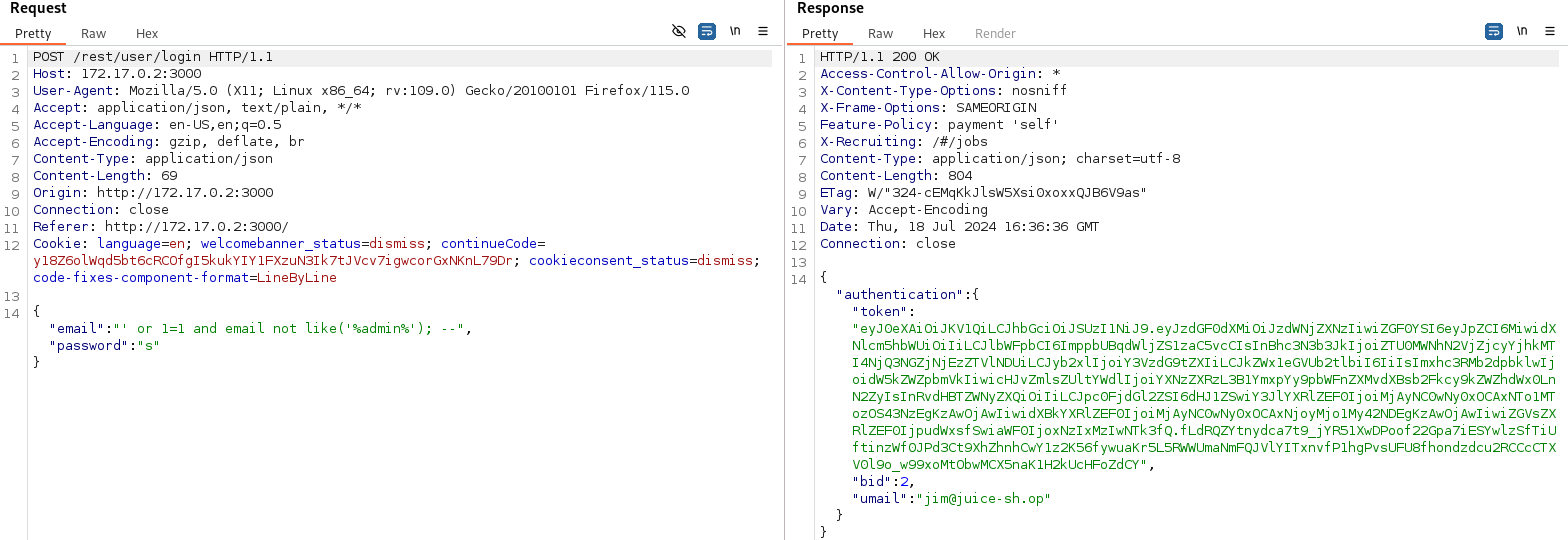
\includegraphics[width=3.73438in,height=2.35768in]{media/image29.png}

\subsection{Esecuzione sul
controllore}\label{esecuzione-sul-controllore}

La CPU funziona tramite il ciclo \textbf{fetch-decode-execute}, nei
microcontrollori si usa l'architettura Harvard che al contrario di
quella Von Neumann memorizza istruzioni e dati in memorie separate
(codice e dati letti/scritti insieme).

Il codice viene eseguito tramite \textbf{super loop}, che ha un
inizializzazione e un ciclo infinito che esegue un task ripetutamente.
Questo approccio semplice la rende \emph{perfetta per lo sviluppo} di
applicazioni ma \emph{non permette una gestione della temporizzazione}
molto accurata.

\subsection{GPIO (General Purpose I/O)}\label{gpio-general-purpose-io}

I microcontrollori normalmente dispongono di una serie di pin,
normalmente general purpose (programmabili per fare input o output).

I pin sono digitali (valore 0 o 1) o analogici (assumono qualsiasi
valore).

\subsubsection{PIN}\label{pin}

Per i pin I/O occorre sempre prestare attenzione ai parametri di
funzionamento, cioè tensione (volt) da applicare o emessa in uscita e la
corrente (Ampere) che può ricevere o fornire.

Per evitare il floating (segnale input senza collegamento, cioè senza
tensione che li porta a captare qualsiasi disturbo) è possibile
equipaggiare i pin con circuiti pull-up.

I \textbf{pin PWM} \emph{emulano in uscita un segnale analogico} a
partire da uno digitale, possibile grazie alla modulazione del duty
cycle (\% di tempo che il segnale è ad 1 rispetto a quella in cui è 0)
di un'onda quadra.

I \textbf{pin IRQ} r\emph{icevono segnali di interruzione} permettendo
al microcontrollore di r\emph{eagire ad eventi e eseguire istruzioni che
non sono} direttamente \emph{nel loop} ma in routine separate.

All'arrivo di una richiesta si sospende l'esecuzione delle istruzioni,
si salva nello stack, restituisce il controllo alla routine di interrupt
(chiamata a interrupt handler o interrupt service routine).

Finito l'interrupt si riprende dal punto di sospensione.

Si possono disabilitare le interruzioni, in questo modo siamo sicuri che
certi parti di codice verranno eseguite senza intoppi, le interrupt
request verranno eseguite quando le interruzioni saranno riabilitate (
se ci dimentichiamo di riabilitarle il sistema potrebbe risentirne);
inoltre le interrupt possono interrompersi fra loro (interrupt nesting).

Se occorre elaborare un segnale analogico bisogna trasformarlo in
digitale tramite l'\textbf{ADC} che mappa il valore continuo in un
valore discreto nel range 0-1023. Un segnale discreto può essere
codificato.

\subsection{Timers}\label{timers}

Per realizzare un comportamento timer-oriented i timer diventano
essenziali per misurare gli intervalli di tempo, gestire i PWM e
realizzare timeout.

Alcuni timer sono:

\begin{itemize}
\item
  \textbf{Watch dog timer}: utilizzato per resettare il circuito in
  situazioni di blocco;
\item
  \textbf{Power management:} permette di utilizzare il circuito con
  diversi livelli di risparmio energetico.
\end{itemize}

\subsection{Protocolli di comunicazione e
bus}\label{protocolli-di-comunicazione-e-bus}

Le interfacce di tipo seriale e parallelo servono per evitare lo scambio
di dati mediante singoli pin, le parallele inviano dati parallelamente
con l'utilizzo di diversi fili invece le seriali inviano dati
sequenzialmente.

\subsubsection{Seriali}\label{seriali}

Ne esistono di due tipologie:

\begin{itemize}
\item
  \textbf{Sincroni}: c'è un clock, aumentano velocità e complessità
  (\(I^{2}\)C e SPI);
\item
  \textbf{Asincroni}: non c'è clock,2 linee (trasmissione e ricezione)
  (USB, RS-485, TTL); i parametri necessari per gestire la comunicazione
  basata su un protocollo prestabilito sono:

  \begin{itemize}
  \item
    \emph{baudRate}: velocità della trasmissione (bps), più è alta più
    possibili errori di trasmissione;
  \item
    \emph{dataFrame}: struttura del pacchetto;
  \item
    \emph{syncBit}: identifica eventuali bit di start e stop del
    pacchetto dati;
  \item
    \emph{parityBit}: serve per error checking (opzionale);
  \end{itemize}
\end{itemize}

Normalmente i bus seriali sono cablati con due linee separate con un
ricevitore (RX) e un trasmettitore (TX) collegati in maniera incrociata
tra due device:

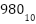
\includegraphics[width=5.26042in,height=3.3125in]{media/image32.png}

Se entrambi i dispositivi possono inviare e ricevere simultaneamente si
ha una comunicazione \emph{FULL-DUPLEX}, se comunicano a turno
\emph{HALF-DUPLEX}. Esiste anche la \emph{Serial Enable LCD}, una
comunicazione seriale basata su singolo cavo.

L'\emph{UART} è il blocco circuitale in grado di convertire i dati da e
verso l'interfaccia seriale mettendola in comunicazione con
l'interfaccia parallela. È asincrono, si appoggia a dispositivi separati
per gestire i flussi di dati e utilizza un bus seriale.

\paragraph{Seriali sincroni}\label{seriali-sincroni}

Abbinando un clock ad un'interfaccia seriale la si rende sincrona,
portando ad avere trasmissioni più rapide (ES: protocolli SPI e
\(I^{2}\)C).

\(I^{2}\)C è nato in Philips, veloce e robusto a due vie che utilizza
l'indirizzamento a 7 o 10 bit e si può arrivare a 3.4Mbit/s. Ha
un'architettura master-slave e più device condividono la SCL (Serial
Clock Line) e SDA (Serial Data Line).

SPI è di Motorola ed è seriale full-duplex, basato su master-slave che
utilizza due linee MOSI (Master Out Slave In) per trasmettere e MISO
(Master In Slave Out) per ricevere; la linea Slave Select è riservata
per la selezione dello slave.

Grazie al Segnale di clock condiviso (SCLK) è sincrono.

In sostanza:

\begin{itemize}
\item
  SPI: + veloce, + semplice, nessuna richiesta di pull-up;
\item
  \(I^{2}\)C: solo 2 linee, indirizzamenti + semplici e aperti.
\end{itemize}

\section{Sistemi SOC e RTOS}\label{sistemi-soc-e-rtos}

I SOC (System On a Chip) sono circuiti integrati in cui un unico chip
contiene un intero sistema operativo (CPU, Chipset, COntroller, Sistema
Video, I/O, Generatore di Clock e regolatori di tensione).

Nei SOC si installano S.O. detti RTOS (Real-Time Operating System) che
permettono la configurazione di sistemi reattivi e completi.

\subsection{Sistemi Operativi}\label{sistemi-operativi}

Nei S.O. moderni hardware e software comunicano attraverso moduli che si
occupano di diverse funzionalità (gestione di: processi, memoria, rete,
ecc), fornendo interfacce che permettono lo scambio di dati e
nascondendo dettagli implementativi tramite l'astrazione.

I S.O sono software di base con lo scopo di gestire hardware e software
ponendosi come mediatore tramite l'utilizzo di API chiamate
\emph{chiamate di sistema}, eseguendo e gestendo i programmi e rendendo
più facile ed efficace l'utilizzo delle risorse attuando algoritmi di
scheduling che gestiscono la concorrenza dei programmi, garantendo
sicurezza e protezione.

La vera struttura hardware viene nascosta al software che vede solo la
macchina virtuale con una vista \emph{top-down} che aumenta la
portabilità dei programmi e semplificando la programmazione delle
applicazioni che potranno essere eseguite su macchine fisiche differenti
(se la macchina virtuale fornisce la stessa interfaccia).

\subsubsection{Interfacce}\label{interfacce}

Ne esistono due principali:

\begin{itemize}
\item
  \textbf{ISA}: Istruction Set Architecture, separa i livelli HW e SW,
  divisa in due parti: \emph{user ISA} che si occupa delle funzionalità
  visibili ai programmi utente e \emph{system ISA} che si occupa delle
  funzionalità del S.O;
\item
  \textbf{ABI}: Application Binary Interface permette l'accesso alle
  risorse HW e ai servizi del sistema ai programmi tramite \emph{user
  ISA} e \emph{System Call Interface} fornite dal S.O.
\end{itemize}

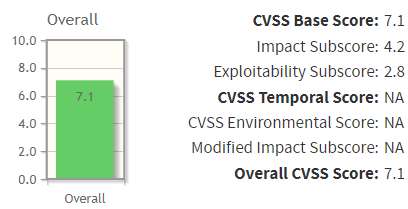
\includegraphics[width=6.26772in,height=2.55556in]{media/image27.png}

Per l'esecuzione dei programmi il S.O. può adottare due costrutti:

\begin{itemize}
\item
  \textbf{Multiprogrammazione} quindi il \emph{caricamento in memoria
  centrale di più programmi e gestendo concorrentemente
  l\textquotesingle accesso all'utilizzo della CPU} \emph{quando i
  programmi utilizzano risorse differenti}.
\item
  \textbf{Multi-tasking} \emph{permette di eseguire programmi
  concorrentemente senza che questi debbano accedere ad altre risorse
  grazie le strategie di schedulazione}; se due task cercano di accedere
  alla stessa risorsa ho una dipendenza relativa ai dati.
\end{itemize}

\subsection{RTOS}\label{rtos}

S.O. real time creati apposta per i sistemi embedded che offrono
compattezza, estrema efficienza nelle gestione risorse e affidabilità.

Non offrono la multi-programmazione e l'esecuzione si limita ad una sola
applicazione ma permette l'esecuzione multi-task.

Questi S.O. devono reagire e rispondere entro determinati range
temporali prestabiliti e rispettare deadline, se le deadline sono sempre
rispettare si dicono \textbf{Hard real-time} e si utilizzano nei sistemi
safety-critical. Se sono ammessi casi in cui le deadline possono non
essere rispettate si dicono \textbf{Soft real-time} e si utilizzano
nell'elettronica di consumo.

Nei sistemi real time \emph{tutto deve essere predicibile}, come il
tempo impiegato da un task, il tempo max per un'azione e la costanza
nella qualità dei cicli richiesti per un'operazione.

\emph{Le interruzioni sono comunque disponibili.}

\subsubsection{Responsiveness e
Overhead}\label{responsiveness-e-overhead}

Al contrario dei microcontrollori, che prediligono un loop con polling
continuo, per verifiche e esecuzioni di funzioni nei RTOS si sfruttano i
context switch che sono più predicibili e non aggiungono overhead al
dispositivo con eventuale calo di prestazione.

\subsubsection{Gestione risorse}\label{gestione-risorse}

Per arbitrare e gestire l\textquotesingle accesso alle risorse vengono
messi a disposizione meccanismi centralizzati, come:

\begin{itemize}
\item
  Allocazione/deallocazione della memoria;
\item
  Semafori e mutex;
\item
  Meccanismi per gestire le sezioni critiche ei suoi problemi.
\end{itemize}

\subsubsection{Semplificazione}\label{semplificazione}

Gli RTOS offrono servizi di astrazione per l'HW e l'utilizzo di
framework e piattaforme per gestire prodotti di terze parti; questo
approccio migliora il lavoro di team e un'agevolazione del debug con la
modulazione del software garantendo manutenibilità ed estensibilità

I RTOS non sono congeniali per applicazioni semplici perchè basterebbe
un'architettura a looping o polling.

\section{Sensoristica}\label{sensoristica}

I \textbf{sensori} sono dispositivi trasduttori che misurano un certo
fenomeno fisico o concentrazione chimica fornendo scala o intervallo;
sono sia digitali che analogici.

In sostanza misurano tutto ciò che ``viene da fuori''.

Il suo scopo principale infatti è quello di misurare, cioè confrontare
due quantità omogenee, stabilendo in che rapporto una quantità incognita
stia rispetto ad un'altra che opera come riferimento.

Gli \textbf{attuatori} producono un effetto sull'ambiente (un led per
esempio) e sono sia analogici che digitali.

Entrambi forniscono segnali analogici quindi continui ad risoluzione
infinita che rappresentano la grandezza fisica continua oppure
codificati in bit o logici (booleani) che rappresentano la grandezza
discreta.

Il segnale analogico per essere elaborato da un calcolatore deve essere
trasformato in digitale tramite un \emph{convertitore ADC}, che campiona
il segnale (vengono presi dei campioni ad intervalli regolari di tempo)
con la \emph{quantizzazione} invece si approssimizza il valore
campionato al più vicino digitale, può produrre un errore nella
misurazione.

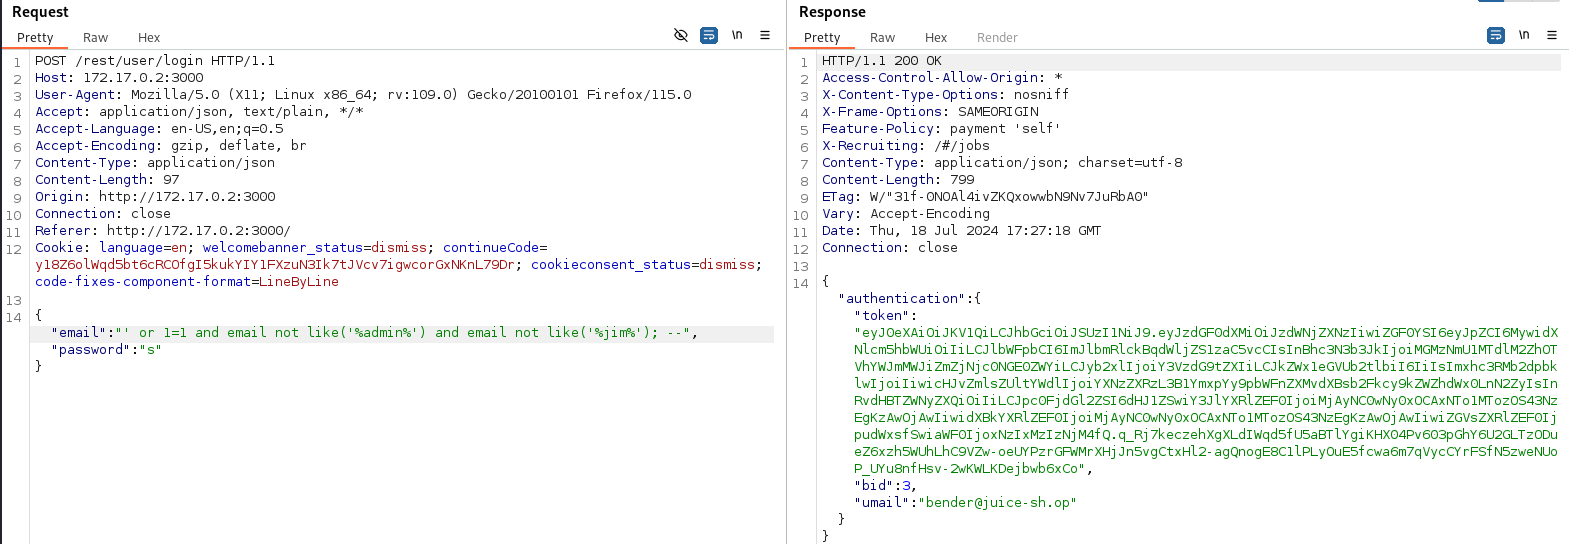
\includegraphics[width=6.26772in,height=2.72222in]{media/image16.png}

\subsection{Misure e incertezze}\label{misure-e-incertezze}

Ogni misura ha errori e/o incertezze, dove \emph{l'incertezza esprime la
dispersione dei valori che verificatasi in misurazioni ripetute si
trasforma in un errore}.

In una misura il risultato è un numero ed una incertezza preceduta dal
simbolo \textbf{±} e con un'unità di misura.

Un errore può essere:

\begin{itemize}
\item
  Sistematico: sempre stessa influenza;
\item
  Casuale:influenza che cambia in grandezza e segno;
\item
  Grossolani: riguardano lo strumento o l'operatore.
\end{itemize}

Se non vengono monitorate le condizioni ambientali possono sorgere
errori casuali, diversamente sono sistematici.

\subsection{Caratteristiche dei
sensori}\label{caratteristiche-dei-sensori}

I sistemi di misura possono essere descritti tramite diverse
caratteristiche divisibili in statiche e dinamiche:

\begin{itemize}
\item
  Statiche: il tempo non influisce sullo strumento, definite dalla
  funzione \(Y\  = F(x)\), con X segnale in ingresso e Y in uscita.
\end{itemize}

\begin{quote}
Sono valutate in una situazione di normale funzionamento, dove la
caratteristica ideale è una retta con pendenza unitaria, ma nella realtà
il comportamento non è ideale (per via di imperfezioni costruttive) e
produce una deviazione di uscita rispetto al ``vero'', questa differenza
è l'errore del sensore.

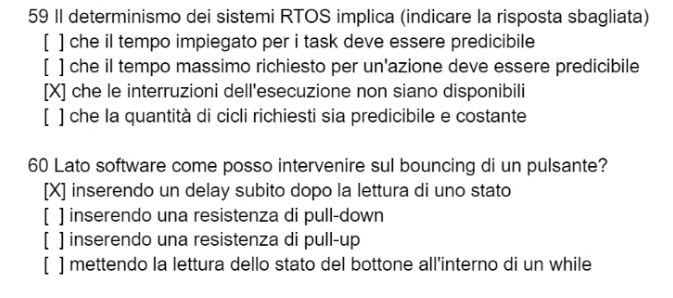
\includegraphics[width=2.29688in,height=1.59654in]{media/image21.png}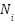
\includegraphics[width=2.51419in,height=1.47773in]{media/image36.png}

Per considerare l'errore bisogna definire \emph{la fascia di incertezza
che rappresenta la massima deviazione della sua retta di riferimento.}

La scomposizione dell'errore nelle sue componenti serve per correggere a
posteriori la misura, altrimenti con la calibrazione o taratura andiamo
a mitigare l'errore sul nascere.

\textbf{Isteresi} cioè la differenza massima tra i valori di uscita
corrispondente ad uno stesso ingresso, ottenuto prima per valori
crescenti, poi decrescenti.

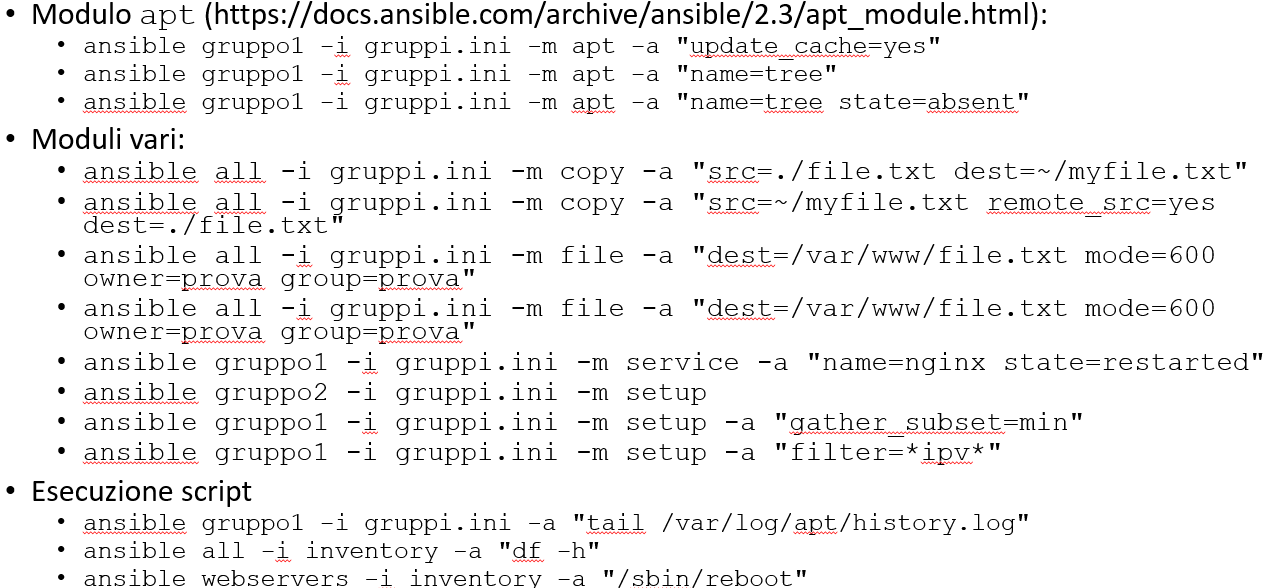
\includegraphics[width=2.45313in,height=1.86256in]{media/image2.png}

\textbf{Ripetibilità} è la capacità di riprodurre la stessa uscita con
lo stesso ingresso consecutivamente e nelle stesse condizioni.

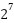
\includegraphics[width=2.35052in,height=1.75683in]{media/image11.png}

\textbf{Linearità}, lo scostamento della curva di taratura della retta
di riferimento, misurata agli estremi è detta terminale, a metà si dice
indipendente e ai minimi quadrati.

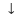
\includegraphics[width=2.20989in,height=1.66907in]{media/image23.png}

\textbf{Risoluzione}: l'ampiezza del passo delle uscite (distanza fra
due uscite consecutive) al variare dell'ingresso in tutto il suo range.

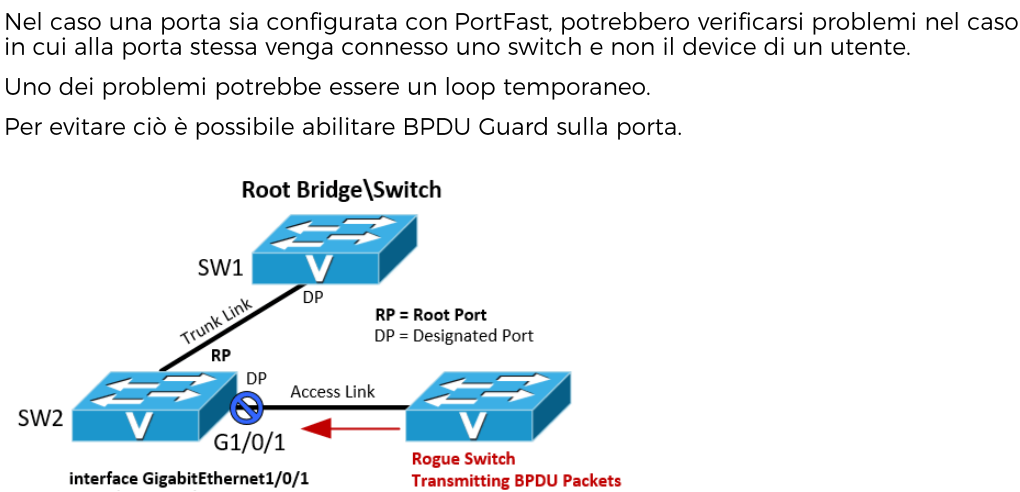
\includegraphics[width=2.25156in,height=1.85037in]{media/image15.png}

\textbf{Sensibilità o guadagno} è la proporzionalità tra valore di
ingresso e valore di uscita, cioè la sensibilità in uscita di un
sensore, rappresenta la pendenza \emph{m} della retta.

\textbf{Offset} rappresenta il segnale in uscita anche in assenza del
segnale di ingresso, è il termine noto \emph{Q} della retta.

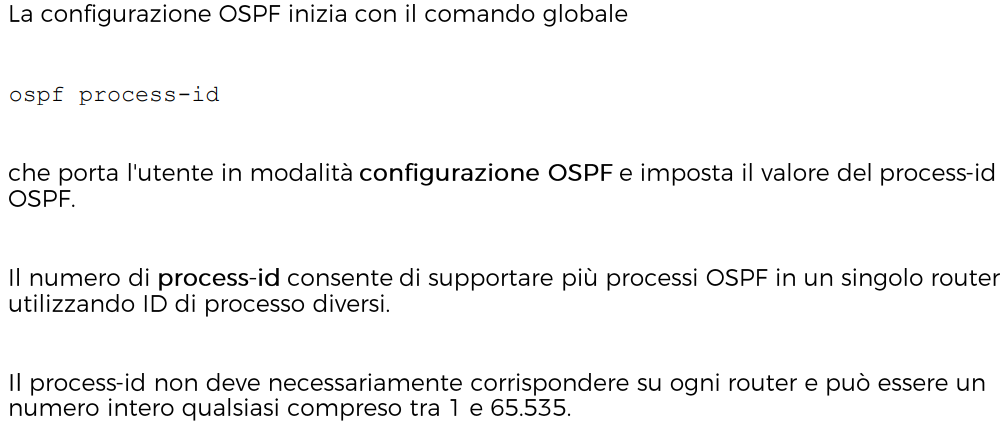
\includegraphics[width=2.53646in,height=1.94874in]{media/image4.png}

\textbf{Accuratezza} è la misura di quanto il valore letto dal sensore
si discordi dal valore corretto, la \textbf{Precisione} descrive quanto
un sensore sia soggetto o meno ad errori accidentali (legata alla
ripetibilità).

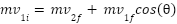
\includegraphics[width=4.27604in,height=1.3851in]{media/image35.png}
\end{quote}

\begin{itemize}
\item
  Dinamiche: il tempo influisce ed è un fattore cruciale, alcune
  caratteristiche sono: \textbf{tempo di risposta} cioè il tempo
  necessario per l'uscita di raggiungere una percentuale specifica del
  valore finale, \textbf{tempo di salita} necessario affinché l'uscita
  vada da prefissato valore ad uno maggiore e \textbf{costante di tempo}
  necessaria affinché l\textquotesingle uscita raggiunga il 63\% del
  valore finale.
\end{itemize}

Il \textbf{guadagno} (K) del trasduttore è la \emph{costante di
proporzionalità fra i valori in ingresso e quelli di uscita prendendo in
esame la caratteristica statica} che idealmente deve essere lineare.

I trasduttori commerciali hanno una caratteristica statica reale che è
leggermente diversa da quella ideale, questo a causa di imperfezioni
costruttive. La qualità del sensore si misura in base a quanto la
caratteristica reale si discosta da quella ideale.

Per i trasduttori lineari la relazione tra la grandezza fisica misurata
e il segnale in uscita è una relazione lineare del tipo: Y = KX (dove K
è il guadagno).

\emph{L'errore di linearità è la massima deviazione dell'uscita del
trasduttore rispetto alla caratteristica lineare che approssima al
meglio quella reale}. La caratteristica lineare viene normalmente
ottenuta secondo il metodo dei minimi quadrati.

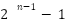
\includegraphics[width=4.70833in,height=2.75in]{media/image10.png}

\subsubsection{Errori di\ldots{}}\label{errori-di}

\textbf{Offset} o errore di fuori zero è il valore che assume l'uscita
del trasduttore quando la grandezza da misurare è nulla.

\textbf{Soglia} corrisponde al più basso livello di segnale rilevabile
dal sensore. Non è necessariamente coincidente con la grandezza da
misurare.

\textbf{Guadagno} descrizione del comportamento dello strumento, fatta
in relazione al tempo, ovvero si descrive il modo di funzionamento nel
caso in cui l'ingresso sia tempovariante (tempo di risposta).

\subsection{Tipi di sensori}\label{tipi-di-sensori}

\subsubsection{Prossimità}\label{prossimituxe0}

Rileva la presenza di oggetti nelle vicinanze della parte sensibile del
sensore (induttiva, magnetica, ottica, ecc) nel raggio della sua portata
nominale (distanza entro la quale il sensore rileva oggetti).

//La parte di sensori leggila nella slides 4 dalla diapositiva 22 a 46

\subsection{Attuatori}\label{attuatori}

Dispositivo che converte dell'energia da una forma ad un'altra,
l'interfacciamento avviene o con la corrente del GPIO o con corrente
maggiore.

\subsubsection{TIpi}\label{tipi}

\textbf{LED}: dispositivi optoelettronici che sfruttano alcuni materiali
semiconduttori in grado di produrre fotoni attraverso un fenomeno di
emissione spontanea; questo li rende altamente efficienti e
particolarmente affidabili.

\textbf{Display LCD}: pannelli formati da due strati di vetro tra i
quali è racchiuso un liquido e numerosi contatti elettrici in grado di
applicare un campo elettrico al liquido, comandando una piccola porzione
di liquido che identifica un pixel.

\textbf{Motori elettrici:} all'interno uno statore ed un rotore che,
producendo un campo magnetico, generano il movimento del rotore. Vi sono
motori di diverso tipo, i più comuni nei sistemi embedded sono:

\begin{itemize}
\item
  \emph{Corrente continua}: rotazione continua ad elevata velocità o
  coppia, controllo della velocità di rotazione. La corrente attraversa
  un avvolgimento nel rotore che genera il campo magnetico;
\item
  \emph{Passo-Passo (Stepper)}: motore brushless che suddivide la
  rotazione in molti step, la posizione può quindi essere controllata
  accuratamente ed hanno un'escursione di 360 gradi;
\item
  \emph{Servo motori}: come per il precedente è possibile pilotare
  l'angolo del rotore ma la posizione è assoluta e non relativa alla
  posizione corrente, escursione di 180 gradi.
\end{itemize}

\subsubsection{Pilotaggio di circuiti
esterni}\label{pilotaggio-di-circuiti-esterni}

Il Relè permette di aprire/chiudere il secondo circuito mediante
l'azione di un elettro-magnete pilotato dal primo circuito.

Possono essere:

\begin{itemize}
\item
  \textbf{NC} (normalmente chiusi);
\item
  \textbf{NO} (normalmente aperti) se senza tensioni in ingresso sulla
  bobina il contatto in uscita risulta ``spento'',
\end{itemize}

Pilotati con diverse tensioni in ingresso e possono gestire tensioni in
uscita.

I fotoaccoppiatori invece si usano principalmente per trasferire un
segnale da un apparato ad un altro tenendoli isolati elettricamente. Un
led interno si attiva, pilotato da un circuito a bassa tensione, e
attiva una fotocellula, chiudendo l\textquotesingle interruttore del
secondo circuito.

\subsubsection{Partitore di tensione}\label{partitore-di-tensione}

\emph{Permette di produrre in uscita una tensione voluta a partire da
una tensione in ingresso più alta}

Viene usato per evitare problemi sui livelli di tensione differenti che
sensori e circuiti hanno, in modo da evitare danni.

\subsubsection{Resistenze di
pull-up/down}\label{resistenze-di-pull-updown}

Sono molto comuni per sopperire all\textquotesingle alta impedenza dei
pin dei device che li può portare ad uno stato di «Floating ».

Si inserisce quindi una piccola resistenza o tra il pin e Vdd
(resistenza di Pull-Up) o tra il pin e Vss (GND o V0) (resistenza di
Pull-Down).

\section{Architetture software}\label{architetture-software}

La progettazione di un sistema embedded è differente da quella dei
sistemi general purpose, infatti vi sono tre aspetti fondamentali
fortemente connessi fra loro:

\begin{itemize}
\item
  Architettura;
\item
  Applicazione {[}requisiti funzionali e non{]};
\item
  Metodologie di sviluppo.
\end{itemize}

Questo tipo di sviluppo è molto complesso e per raggiungere un buon
prodotto occorrono analisi, simulazioni alternate con l'uso di prototipi
dove la simulazione non fornisce valori accettabili e strumenti avanzati
per il testing dell'hardware.

Inoltre si consiglia l'utilizzo di una metodologia ibrida, in grado di
integrare metodologie di sviluppo software e hardware.

\subsection{Metodologie}\label{metodologie}

\subsubsection{Co-design}\label{co-design}

Utilizzata quando sono presenti componenti hardware e software insieme,
mira a ottimizzare il processo di progetto andando ad aumentare la
produttività e accorciando i tempi di sviluppo con il riuso dei
componenti.

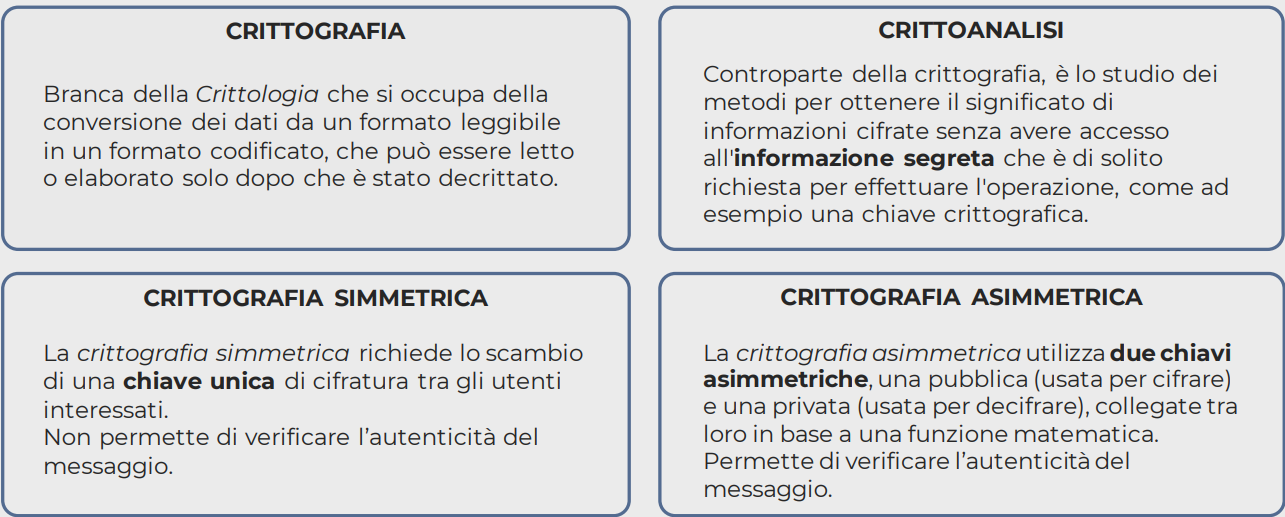
\includegraphics[width=6.26772in,height=1.70833in]{media/image20.png}

\textbf{Co-Specifica}: si analizza e si fa una specifica insieme;

\textbf{Co-Partizionamento}: divisione componenti tra hardware e
software, un buon compromesso mitiga costi e ottimizza le prestazioni;

\textbf{Co-Sintesi}: sviluppo componenti, diviso in 4 fasi:

\begin{itemize}
\item
  \emph{comunicazione}: interfacciamento tra HW e SW;
\item
  \emph{personalizzazione delle specifiche}: metodi di comunicazione per
  permettere l'interfacciamento;
\item
  \emph{specifiche HW;}
\item
  \emph{specifiche SW};
\end{itemize}

\textbf{Co-Scheduling}: assegnamento timing di esecuzione per ridurre la
latenza al minimo;

\textbf{Co-Simulazione}: verifica funzionalità hardware e software;

\textbf{Co-validation}: verifica del sistema e diversi livelli di
astrazione.

\subsubsection{Modello a cascata}\label{modello-a-cascata}

Modello classico e vecchio stile, dove ogni fase genera un output
necessario per quella successiva. Gestione semplice per progetti piccoli
ma pericoloso per progetti più complicati e lunghi rendendo impossibile
effettuare modifiche ai livelli superiori.

\subsubsection{Modello a spirale}\label{modello-a-spirale}

In realtà è un metamodello creato da Barry Boehm e rappresenta diversi
cicli di vita, si basa su quattro fasi: \emph{pianificazione, analisi,
sviluppo e verifica}.

\emph{Il raggio delle fasi è il costo accumulato} (+ è alto + il costo
aumenta) e la dimensione angolare il progresso, favorisce uno sviluppo
costante e definito.

\subsubsection{Metodologia agili
{[}agiail{]}}\label{metodologia-agili-agiail}

Usata dalla Vem, al centro c'è il cliente che si incontra ogni due
settimane per mostrare i progressi fatti e verificare che siano in linea
con quello che il cliente vuole.

Basato sul metodo ``Scram'', ma con regole meno ferree, dove si divide
il progetto in sprint (massimo 3 settimane) dove si lavora senza
sottoteam e ogni membro del progetto sceglie un task da sviluppare
(scelto nello sprint planning); ogni task è creato dal capo progetto e
sono molto base.

A fine sprint si mostra al cliente le nuove funzionalità nello sprint
review; successivamente si ricomincia con lo sprint planning dove creo e
distribuisco i task nuovi e decido quali task vecchi non completati
portare allo sprint successivo.

\subsection{Modellazione}\label{modellazione}

Uno dei momenti più importanti durante lo sviluppo di un software poiché
fondamentale per rappresentare il sistema definendo soluzioni più
astratte offrendo migliore comprensione, estensibilità, portabilità e
modularità.

Attraverso dei modelli ben definiti e basati su paradigmi di
programmazione è possibile concettualizzare il sistema rappresentandone
gli aspetti salienti ed astraendo i meno significativi.

La modellazione su MCU avviene tramite un controllore che contiene la
logica di controllo e gestisce le risorse, è la parte normalmente attiva
con un modello a loop di controllo.

Gli elementi controllati invece modellano le risorse gestite dal
controllore per svolgere i compiti, contengono le funzionalità utili al
controllore e sono tipicamente passivi, solo la parte riusabile.

\subsection{Paradigma OO}\label{paradigma-oo}

Paradigma ad oggetti offre un buon livello di astrazione con proprietà
come modularità, incapsulamento e meccanismi per il riuso e
l\textquotesingle estensibilità.

Inoltre permette di avere un supporto naturale alla modellazione
software di oggetti reali.

Il modello a loop ci sono alcuni limiti, infatti i loop continuano ad
essere eseguiti anche quando non vi sono cambiamenti di input
(efficienza) e se il ciclo è piuttosto complesso a livello
computazionale si possono introdurre dei ritardi, perdendo eventuali
variazioni che vengono compiute durante l'elaborazione (reattività).

Il controller del modello oo non è una classe ma un \textbf{agente},
ovvero:

\emph{Entità attiva dotata di un flusso di controllo logico autonomo.
progettato per svolgere uno o + task che richiedono di elaborare
informazioni provenienti da input dei sensori e di agire su attuatori in
output, comunicando con altri agenti}.

\subsection{Macchine a stati finiti}\label{macchine-a-stati-finiti}

Modello di sistema a dinamica discreta, dove \emph{ogni input viene
mappato in un output}, a seconda del suo stato corrente ad ogni reazione
rilevata, con un numero finito di stati possibili.

\textbf{Stato di sistema}: condizione in cui si trova in un certo
istante temporale, ovvero l'insieme di tutte le attività passate, che
determinano la reazione del sistema agli input futuri.

\textbf{Reazione}: step che il sistema effettua, istantanee e scatenate
dall\textquotesingle ambiente o da eventi.

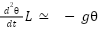
\includegraphics[width=6.26772in,height=3in]{media/image31.png}

Le macchine a stati finiti possono essere:

\begin{itemize}
\item
  \textbf{Asincrone}: cioè event triggered, dove la reazione (o
  transizione) avviene a fronte di un evento in input;
\item
  \textbf{Sincrone:} cioè time triggered, dove le reazioni avvengono ad
  intervalli regolari di tempo, per questo motivo questo tipo di
  macchine sono adatte alla gestione di sistemi time-oriented.
\end{itemize}

\begin{quote}
La lettura di un input con un certo periodo di tempo è detto
\emph{campionamento}, se si sceglie bene il periodo di campionamento è
possibile non perdere eventi e mantenere la reattività al costo di
risorse vista la rapidità del campionamento; il \emph{MEST} (Minimum
Event Separation TIme) è l'intervallo più piccolo che può esserci fra
due eventi di input quindi scegliendo un periodo più piccolo del MEST
rileveremo tutti gli eventi.

La \emph{latenza} è il tempo che intercorre tra l'evento di input e la
generazione dell'output.
\end{quote}

\subsection{Task}\label{task}

\subsubsection{Organizzazione task
concorrenti}\label{organizzazione-task-concorrenti}

L'architettura a task concorrenti nasce dalla necessità di modellare e
progettare applicativi articolati dove è fondamentale decomporre e
modularizzare le funzionalità.

Ogni task ha un compito, un'unità di lavoro e il suo comportamento è
descritto da una macchina a stati; dove il comportamento di tutti i task
è l'insieme delle varie macchine a stati.

I task possono essere suddivisi in sotto-task in maniera ricorsiva
aumentando la modularità portando ad un sistema chiaro, manutenibile,
estendibile e riusabile.

Bisogna ricordarsi che i task sono fra loro concorrenti e le loro
dipendenze vanno gestite mediante forme di coordinazione cooperative o
competitive.

La metodologia cooperativa usa scheduling di tipo round-robin che è più
semplice ed è privo di corse critiche, a scapito di un loop infinito in
uno dei task che può portare gli altri in una situazione di starvation.

\subsubsection{Dipendenze task}\label{dipendenze-task}

Non riuscendo a garantire un\textquotesingle indipendenza completa
esistono forme di dipendenza:

\begin{itemize}
\item
  Temporale: per far partire un altro task bisogna aspettare che l'altro
  finisca;
\item
  Producer/Consumer: un task deve aspettare l\textquotesingle output di
  un altro;
\item
  Relative ai dati: c'è una risorsa in comune, bisogna aspettare che
  l'altro task la liberi.
\end{itemize}

Nelle macchine a stati l'interleaving delle azioni non avviene.

\subsubsection{Comunicazione task}\label{comunicazione-task}

Il caso più semplice è utilizzare una variabile globale, così si ha una
comunicazione sincrona. C'è la possibilità di gestire i messaggi in
maniera asincrona utilizzando per ogni task una coda.

\subsection{Scheduling e prestazioni}\label{scheduling-e-prestazioni}

Per ogni task è necessario valutare la loro durata per evitare
malfunzionamenti, si possono definire eccezioni di overrun quando il
tempo di esecuzione delle azioni oltrepassa il periodo pre stabilito
andando a ``rubare'' tempo di esecuzione al task successivo (timer
overrun nel caso di scheduler interrupt-driven).

È possibile definire se si verificherà un overrun analizzando il codice
per stimare il Worst-Case Execution Time (con task che usano periodi
diversi bisogna considerare il WCET con degli iper-periodi).

\(U\  = \ (tempo\ utilizzo\ per\ task/\ tempo\ totale)\ *\ 100\%\)

Ottenendo un valore \textgreater100\% si verificherà un overrun.

\textbf{Jitter}: ritardo che intercorre dal momento che un task è pronto
per essere eseguito e il momento in cui viene effettivamente eseguito,
dando priorità ai task con periodo piccolo minimizziamo il jitter medio.

\textbf{Deadline}: intervallo di tempo entro il quale un task deve
essere eseguito dopo essere diventato ready.

\subsubsection{Priorità}\label{priorituxe0}

Per priorità si intende l'ordinamento con cui lo scheduler esegue i
task. Normalmente vi possono essere due tipologie di scheduler:

\begin{itemize}
\item
  Priorità statica: ogni task ha un livello di priorità che non cambia
  durante l'esecuzione, si usa la policy shortest-deadline first a meno
  che la deadline non sia uguale altrimenti si passa alla
  shortest-period first;
\item
  Priorità dinamica: la priorità è determinata in esecuzione e la si da
  a chi ha una deadline più vicina alla fine.
\end{itemize}

\subsubsection{Preemptive e cooperativi}\label{preemptive-e-cooperativi}

Sono due tipi di scheduler, il primo può togliere il processo ad un task
in esecuzione prima che abbia completato; il secondo aspetta finché il
task non sia stato portato a termine ed è utilizzato per realizzare le
macchine a stati finiti.

\subsection{Architetture su eventi}\label{architetture-su-eventi}

A basso livello le interruzioni di input rappresentano eventi che
gestiscono meglio le risorse ed evitano polling.

Si possono utilizzare gli eventi anche per realizzare architetture ad
eventi di alto livello come pattern-observer o macchine a stati finiti
asincrone.

\subsubsection{Pattern-observer}\label{pattern-observer}

Si sfruttano le interruzioni per far si che all'occorrenza di
un'interruzione si chiamino i listener.

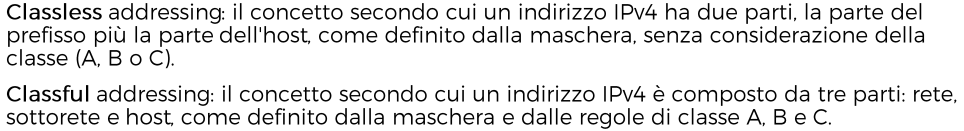
\includegraphics[width=6.26772in,height=1.93056in]{media/image6.png}

\subsubsection{Macchine a stati finiti
asincrone}\label{macchine-a-stati-finiti-asincrone}

Sfruttano le interruzioni per realizzarle, la valutazione delle reazioni
avviene a seguito di un evento, non esiste il periodo anche se l'evento
può essere di tipo temporale.

\section{IOT}\label{iot}

Coniato da Kevin Ashton nel `99, automatizzare l'inserimento dei dati
inerenti al mondo fisico in Internet con sensori con l'ipotesi di un
futuro interconnesso.

Definizione standard:

\emph{``Things having identities and virtuale personalities operating in
smart spaces using intelligent interfaces to connect and communicate
within social, environmental, and user contexts''}

resto nelle slides

\section{Comunicazione}\label{comunicazione}

In ottica IoT la connessione alla rete può essere:

\begin{itemize}
\item
  Diretta: si ha un modulo connessione;
\item
  Indiretta: usando un gateway, usando un sistema terzo.
\end{itemize}

\subsection{Wireless}\label{wireless}

Da non confondere con il WiFi perchè il wireless comprende il WiFi e
tutto ciò che non usa fili per la comunicazione, in sostanza la
radiocomunicazione.

Sfruttando canali radio possiamo trasmettere dati attraverso segnali
elettromagnetici che appartengono alla frequenza radio dello spettro
elettromagnetico; \emph{tali comunicazioni sono satellitari o
terrestri.}

\subsection{Sistema
radiocomunicazione}\label{sistema-radiocomunicazione}

Composto da:

\begin{itemize}
\item
  Canale trasmissivo: tutto ciò che serve per trasmettere;
\item
  Modem: codifica da bit-segnale a elettrico e viceversa;
\item
  Codec: codifica e decodifica digitalmente un segnale.
\end{itemize}

La rete può essere:

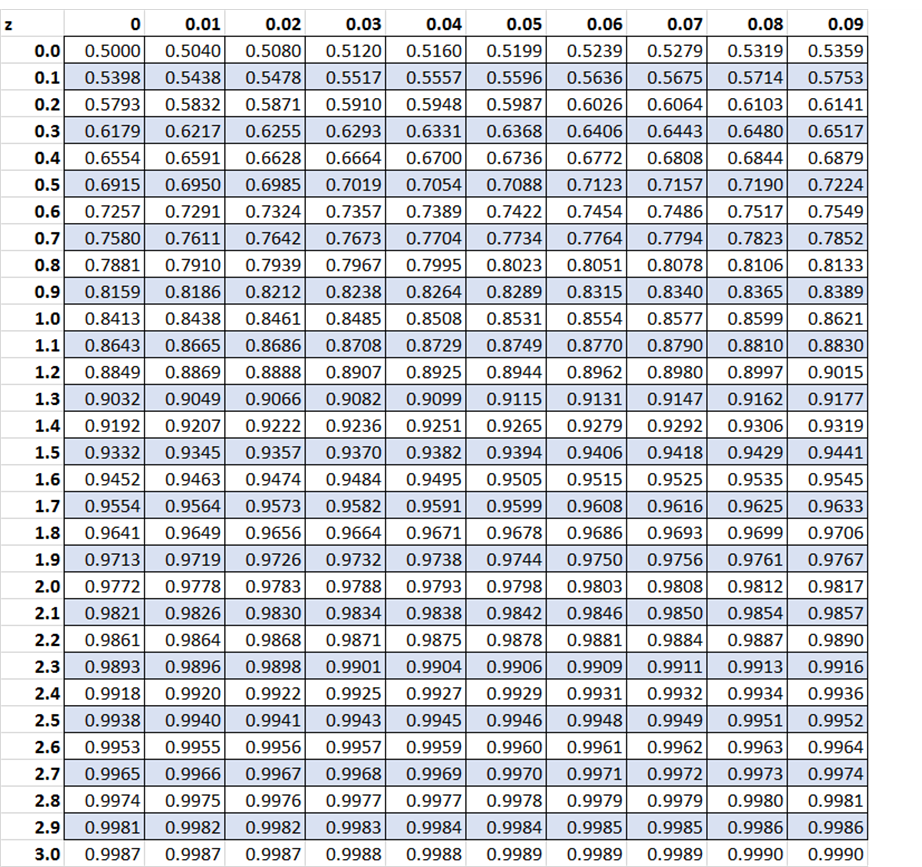
\includegraphics[width=3.04688in,height=2.27567in]{media/image9.png}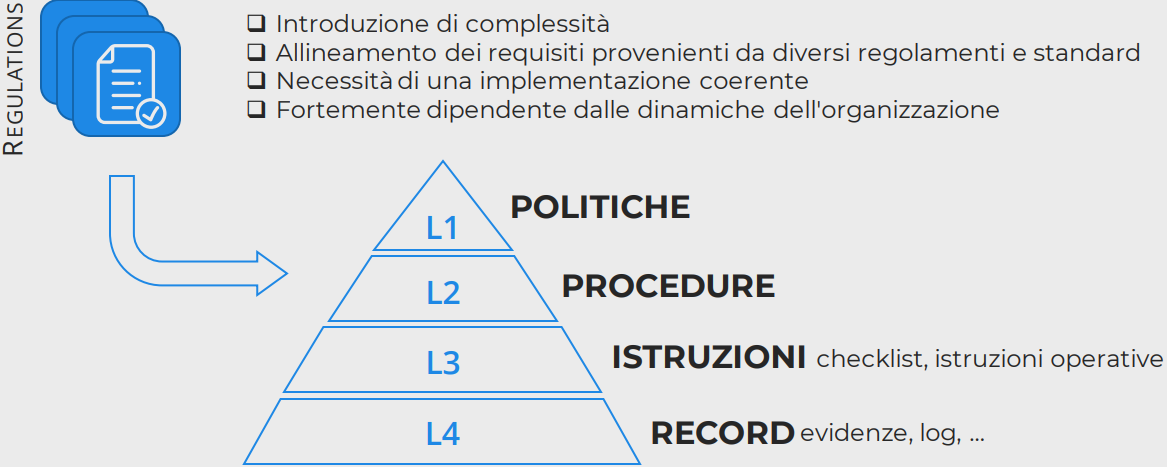
\includegraphics[width=3.09917in,height=1.98815in]{media/image18.png}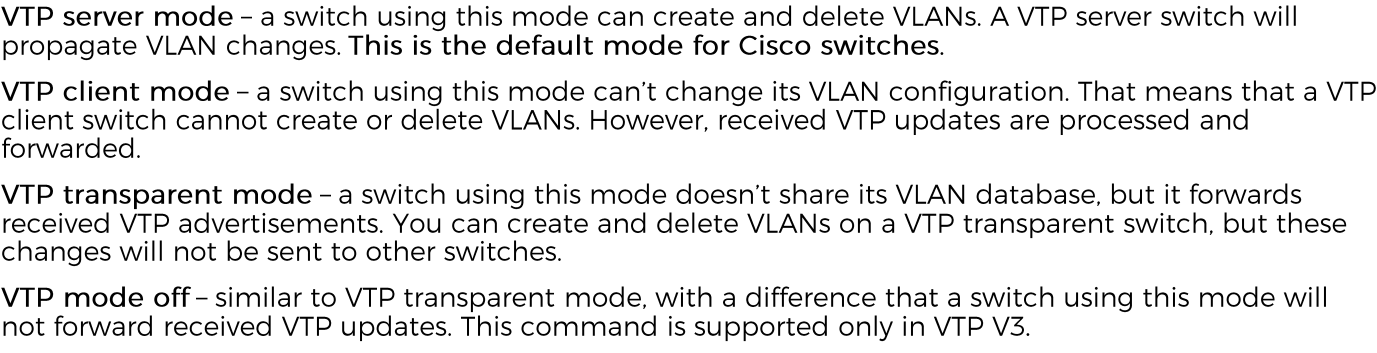
\includegraphics[width=3.15448in,height=2.12356in]{media/image22.png}

\subsubsection{WiFi}\label{wifi}

Standard IEEE 802,11x, supportato da IP, TCP, UDP.

Data rate elevato con un range di 150m, frequenza 2,4 o 5 GHz e con
prestazioni non favorevoli per i sistemi embedded.

\subsubsection{Reti cellulari}\label{reti-cellulari}

Standard evoluti dal GPRS a LTE, data rate che può essere alto o basso
in base allo standard, consumi abbastanza alti e range dell'ordine dei
chilometri.

Successivamente è nato il Narrow Band IoT che utilizza le reti cellulari
ma con copertura altissima e consumi ridotti a scapito del data rate.

\subsubsection{Sistemi RF}\label{sistemi-rf}

Interfacce via radio con data rate a 1 Mbps, range elevati, frequenza di
2,4 GHz e senza supporto di protocolli ad alto livello.

\subsubsection{Bluetooth}\label{bluetooth}

Protocollo 802.15.1, sfrutta la scoperta dinamica di dispositivi entro
10 metri di raggio, costi di produzione e energia bassi, frequenze
libere e con \emph{il frequency hopping} commuta la banda e
\emph{permette di ottimizzare l'utilizzo della frequenza}.

La rete del BT è detta piconet basata sull'architettura master-slave
dove ogni dispositivo comunica con 7 slave e questi slave comunicano in
maniera sincronizzata (grazie al clock master) uno per volta con il
master. Più piconet connesse insieme sono dette scatternet, dove gli
slave possono appartenere a più reti ma il master può essere slave solo
di una sola piconet.

\subsubsection{ZigBee}\label{zigbee}

Il protocollo IEEE 802.15.4, si basa su uno standard di comunicazione e
ne vuole definire uno complementare al WiFi (quindi personale e a basso
costo/velocità), il ZigBee usa questa specifica con comunicazioni entro
10 metri, transfer rate di 250 kbits e utilizzo frequenze 868/915/2450
MHz.

La rete è composta da FFD (coordinatore che parla con tutti) e RFD
(parla solo con il FED).

Il Zigbee è ideato per l'IoT con basso consumo e basso costo, i
dispositivi si dividono in:

\begin{itemize}
\item
  ZigBee Coordinator (ZC): è un ponte fra reti, solo uno per rete e
  tiene le chiavi di sicurezza {[}FFD{]};
\item
  ZigBee Router (ZR): trasmettono dati fra dispositivi {[}FFD{]};
\item
  ZigBee End Device (ZED): parla solo con coordinatore e router
  {[}RFD{]}
\end{itemize}

\subsubsection{LoraWAN}\label{lorawan}

Poca potenza ma grossa area di copertura, costo energetico basso e
utilizzo frequenze radio.

Struttura con topologia a stella avente un gateway per connettersi ad
internet che comunica con un network server (di solito in cloud) che
gestisce i downlink e gli end device possono connettersi a più gateway.

Usando bande libere il protocollo ha dei duty-cycle, cioè un periodo di
tempo per usare la banda, in sostanza il data rate è limitato\emph{.}

\emph{Se aumenta il data rate ci sarà più velocità di trasmissione a
scapito dello spreading factor} (portata delle trasmissioni).

Con spreading factor + alti occorrono pacchetti più piccoli e consumi
più alti.

La comunicazione LoraWAN è bidirezionale con classi di device diverse:

\begin{itemize}
\item
  Classe A: il device di campo inizia sempre a comunicare e solo dopo si
  può rispondere entro una finestra temporale;
\item
  Classe B: come nella classe precedente ma si aprono anche finestre di
  ricezione schedulate;
\item
  Classe C: finestra sempre aperta a meno che non ci sia una
  trasmissione in corso.
\end{itemize}

Bisogna sempre ricevere un uplink prima di inviare un downlink.

\subsubsection{RFID}\label{rfid}

Tracking a distanza tramite tag che hanno un id univoco, i tag possono
essere: passivi (non alimentato), attivo (ha batterie e comunica in
broadcast), BAP (invia informazioni solo se sollecitato).

\subsubsection{NFC}\label{nfc}

Fornisce connettività radio bidirezionale a corto raggio, quando si
accostano i'initiator e il target viene creata una rete peer-to-peer.

\subsubsection{Beacon}\label{beacon}

\emph{Basata sul BLE} utile per localizzazione indoor, si usa un device
detto beacon a basso consumo che trasmette di continuo il suo ID.

\subsection{Middleware}\label{middleware}

Struttura di riferimento per la standardizzazione della connettività via
Internet dei device IoT.

Il loro scopo è fornire interoperabilità (\emph{capacità di un sistema o
di un prodotto informatico di cooperare e di scambiare informazioni})
tramite supporto a protocolli di alto livello, discovery dinamico,
aggiornamenti, disconnettere dispositivi problematici, fornire supporto
per la memorizzazione, scalabilità e sicurezza.

Si hanno diversi livelli:

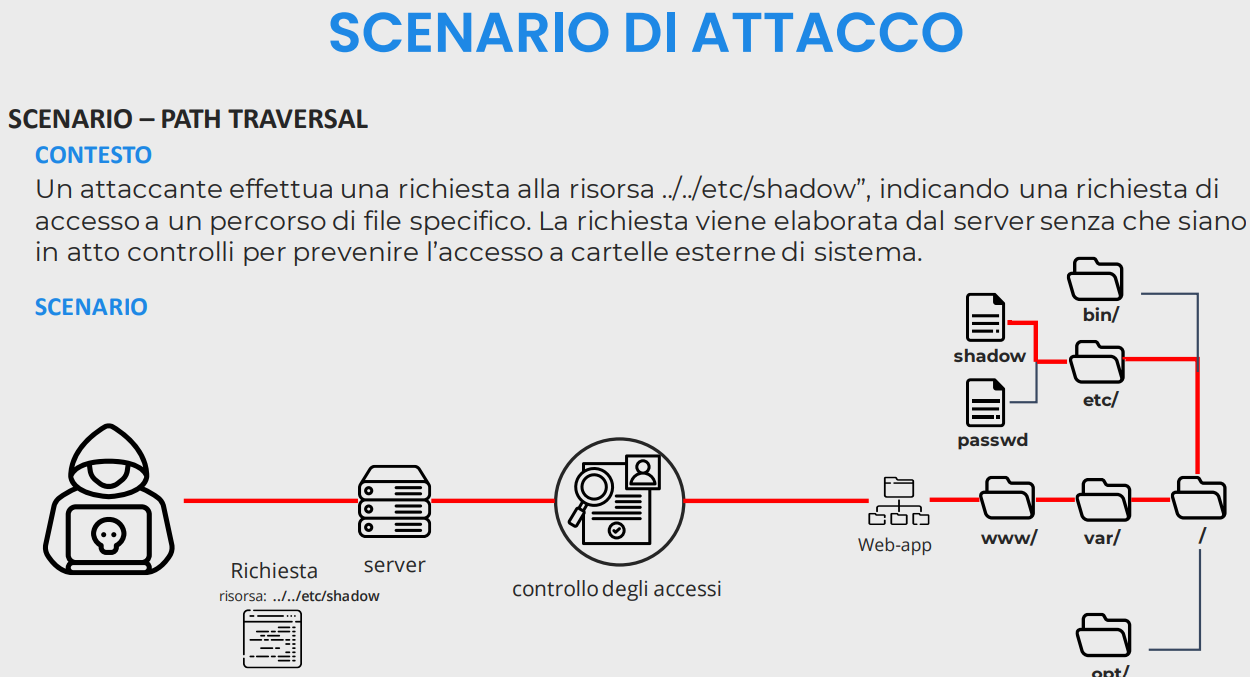
\includegraphics[width=4.70141in,height=3.03872in]{media/image30.png}

Dove:

\begin{itemize}
\item
  \textbf{Event processing}: rileva gli eventi e li processa;
\item
  \textbf{Aggregation}: aggrega e gestisce le comunicazioni e fa da
  ponte fra i vari protocolli;
\item
  \textbf{Comunication}: diversi protocolli possono essere utilizzati,
  http, MQTT, CoAP, XMPP;
\item
  \textbf{Devices}: Dispositivi di vario tipo con o senza connessione
  diretta, identificati a livello HW.
\end{itemize}

\subsection{MQTT}\label{mqtt}

Protocollo a scambio di messaggi \emph{publish-subscribe}, basato sul
modello broker.

Vantaggioso per il suo basso overhead, possibilità di funzionare su
diversi protocolli (TCP, ZigBee) e con anche la presenza di firewall e
garantisce la bontà dei messaggi tramite QOS.

Il QOS ha tre livelli:

\begin{enumerate}
\def\labelenumi{\arabic{enumi}.}
\setcounter{enumi}{-1}
\item
  \textbf{At most once}: viene inviato il messaggio, non importa chi e
  se qualcuno lo legge, per questo detto \emph{fire and forget};
\item
  \textbf{At least once}: c'è la sicurezza che arrivi a destinazione
  almeno una volta;
\item
  \textbf{Exactly once}: il messaggio arriva una sola volta.
\end{enumerate}

\subsection{CoAP}\label{coap}

Basato su HTTP con approccio client-server utilizzando UDP.

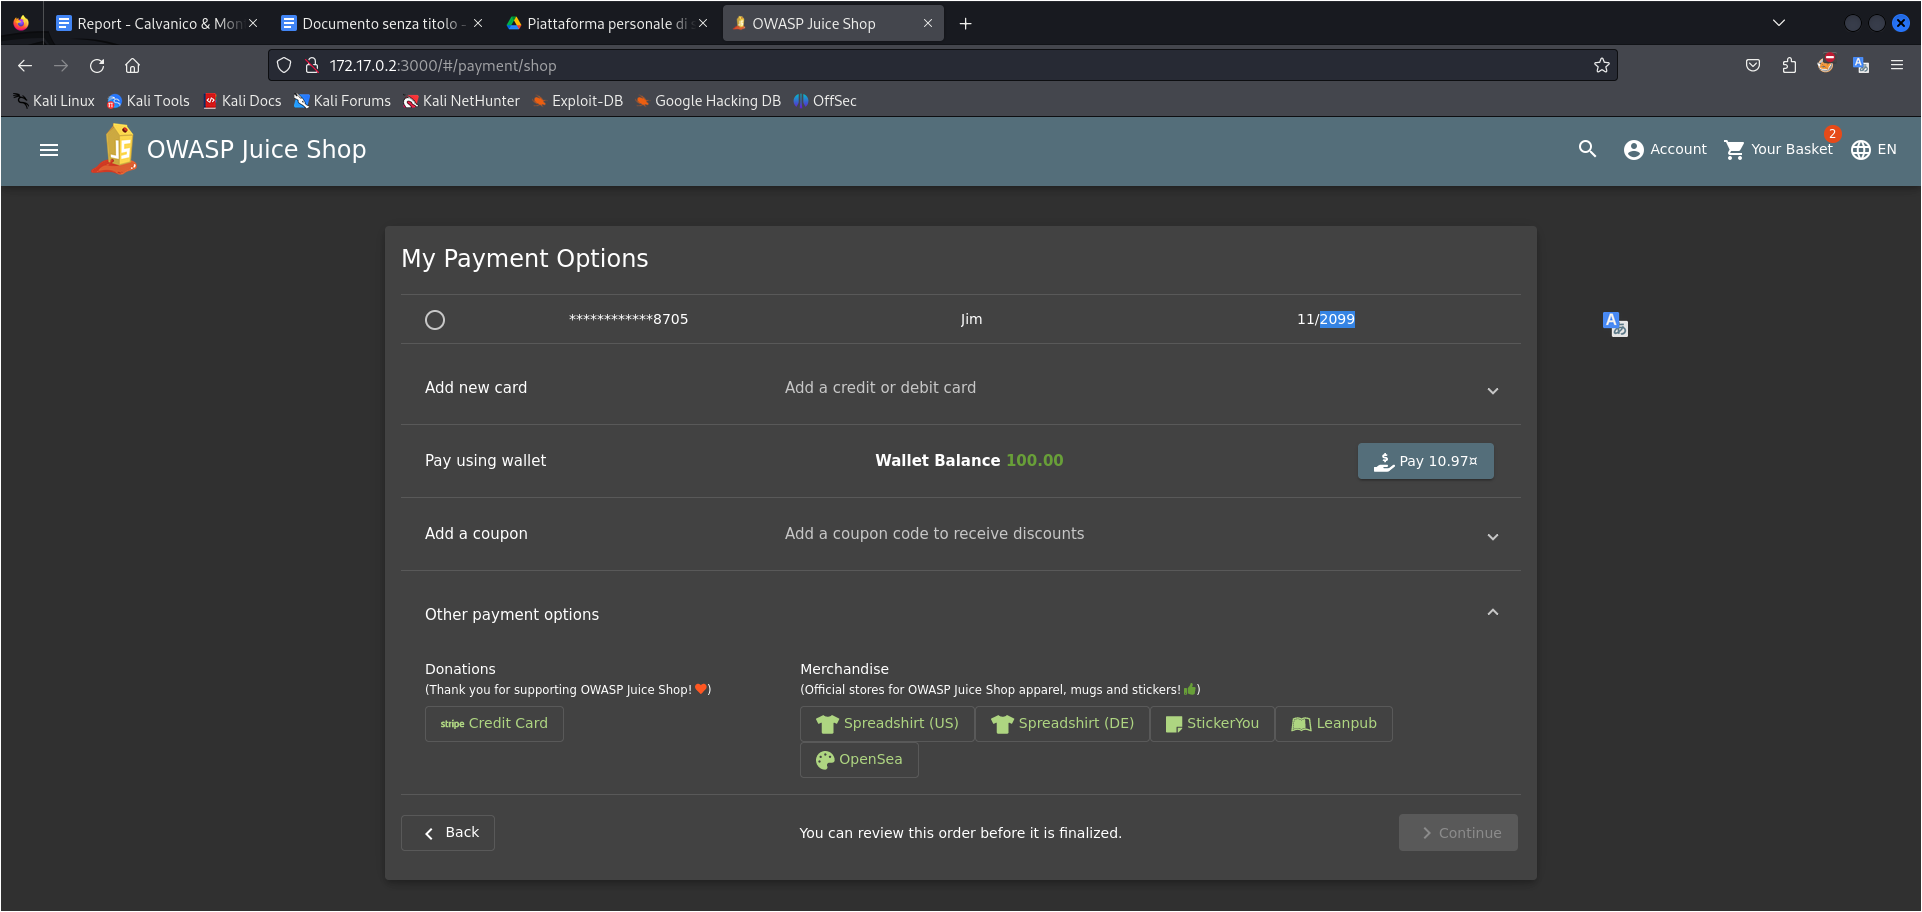
\includegraphics[width=3.52604in,height=2.15545in]{media/image12.png}

\subsection{XMPP}\label{xmpp}

Basato su scambio di messaggi con struttura message-brokers. Supporta
anche altri metodi come il point-to-point, il request-response e
l\textquotesingle asyncronous message, costruendo federazioni di server
XMPP possiamo ottimizzare la scalabilità.

\subsection{Modelli di comunicazione}\label{modelli-di-comunicazione}

\subsubsection{A scambio di messaggi}\label{a-scambio-di-messaggi}

Comunicazione tramite invio e ricezione di messaggi utilizzando send o
receive.

Possono essere:

\begin{itemize}
\item
  \textbf{Diretta}: comunicazione diretta fra processi utilizzando un
  identificativo univoco;
\end{itemize}

\begin{quote}
\textbf{o}
\end{quote}

\begin{itemize}
\item
  \textbf{Indiretta}: sfruttando canali di comunicazione.
\end{itemize}

\begin{itemize}
\item
  \textbf{Sincrona}: la send va a buon fine quando il messaggio è stato
  recepito tramite receive;
\end{itemize}

\begin{quote}
\textbf{o}
\end{quote}

\begin{itemize}
\item
  \textbf{Asincrona}: la send va a buon fine quando il messaggio viene
  inviato.
\end{itemize}

\begin{itemize}
\item
  \textbf{Descrizione dei messaggi.}
\end{itemize}

Non bisogna sottovalutare la bufferizzazione dei messaggi, che nel caso
asincrono è fondamentale. Nel caso il buffer si riempia bisogna gestire
il comportamento della send scegliendo fra i seguenti meccanismi:

\begin{itemize}
\item
  \textbf{La send fallisce} con scarto del messaggio;
\item
  \textbf{La send si blocca} finchè non c'è disponibilità nel buffer;
\item
  \textbf{La send ha successo} e si riscrive il messaggio nel buffer più
  nuovo o vecchio.
\end{itemize}

Per la rappresentazione del messaggio si usa un linguaggio condiviso da
tutti come Json o XML e adottare ontologie (sintassi e strutture
comuni).

\subsubsection{Publish-subscribe}\label{publish-subscribe}

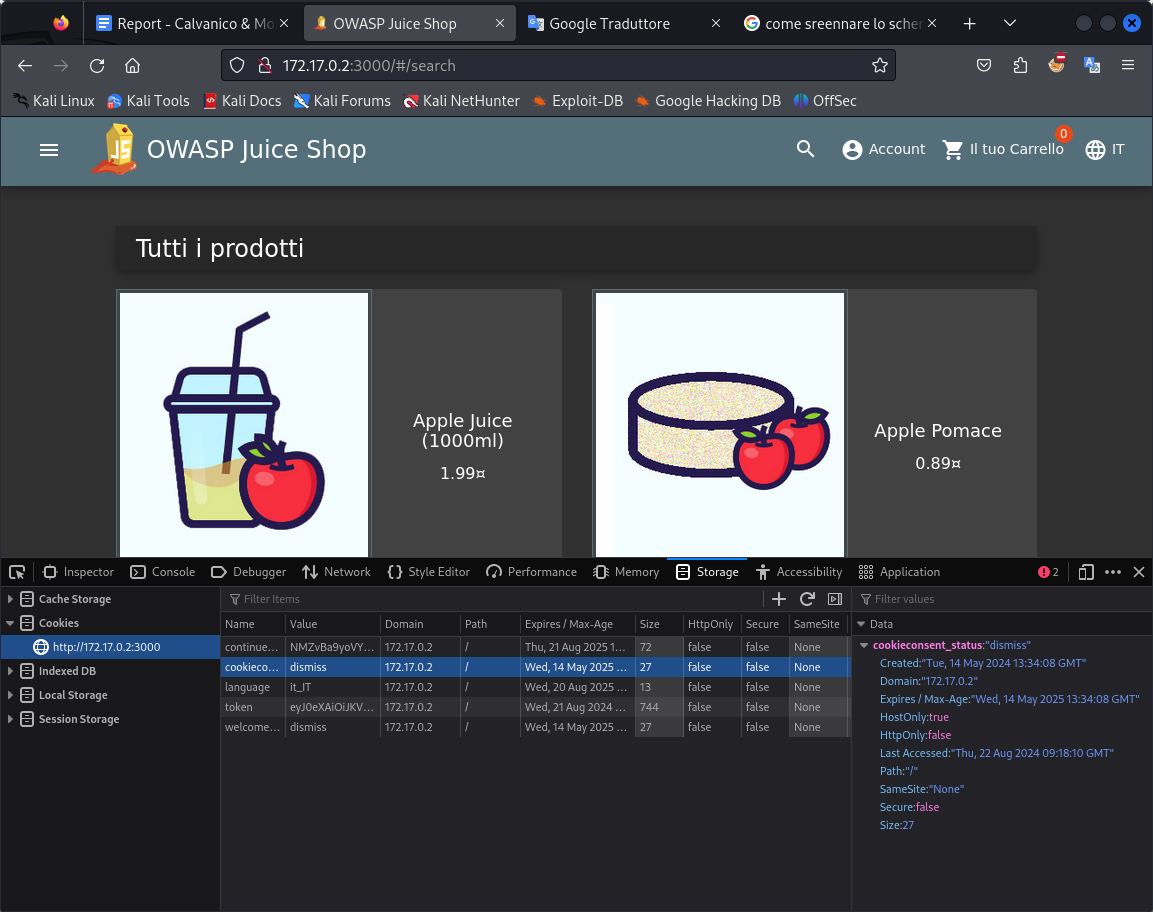
\includegraphics[width=6.26772in,height=3.05556in]{media/image25.png}

Utilizzato nelle strutture ad eventi e composto da:

\begin{itemize}
\item
  \textbf{Topics}: canali in cui è possibile inviare dei messaggi e che
  è possibile «osservare»;
\item
  \textbf{Publisher}: possono inviare messaggi sui topics;
\item
  \textbf{Subscriber}: si registrano ai topics per ricevere tutti i
  messaggi pubblicati su questi.
\end{itemize}

\section{Domande esame}\label{domande-esame}

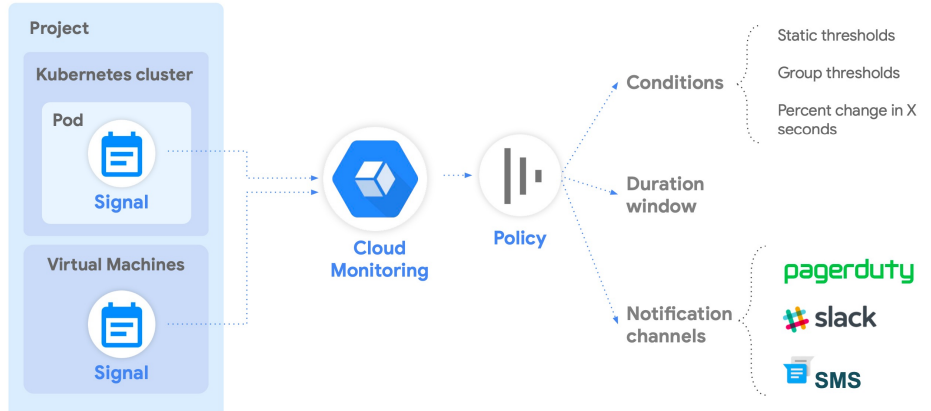
\includegraphics[width=3.96875in,height=3.57292in]{media/image28.png}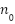
\includegraphics[width=6.26772in,height=2.56944in]{media/image17.png}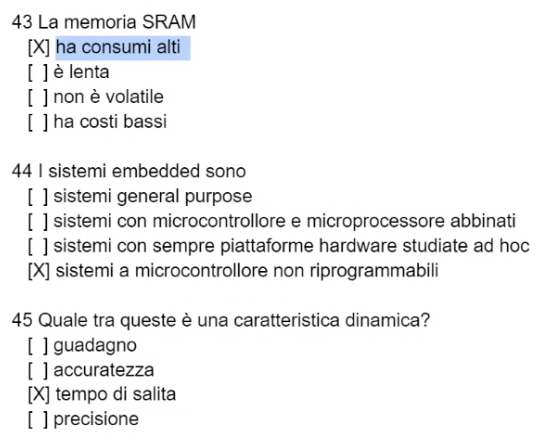
\includegraphics[width=6.26772in,height=1.20833in]{media/image8.png}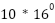
\includegraphics[width=6.26772in,height=3.27778in]{media/image24.png}

Nella domanda 30 la risposta giusta è: serve un server NTP (e non PTN)
per questo sono tutte sbagliate !!!

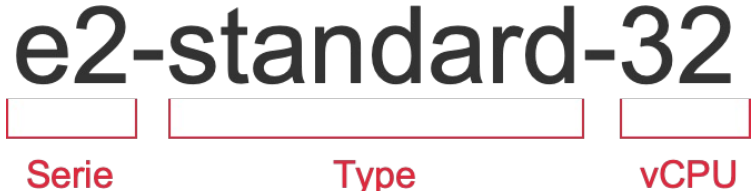
\includegraphics[width=6.26772in,height=3.44444in]{media/image33.png}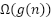
\includegraphics[width=6.26772in,height=4.90278in]{media/image34.png}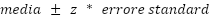
\includegraphics[width=6.26772in,height=1.27778in]{media/image1.png}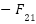
\includegraphics[width=5.70833in,height=4.58333in]{media/image14.png}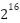
\includegraphics[width=6.19792in,height=3.61458in]{media/image3.png}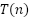
\includegraphics[width=6.26772in,height=2.80556in]{media/image5.png}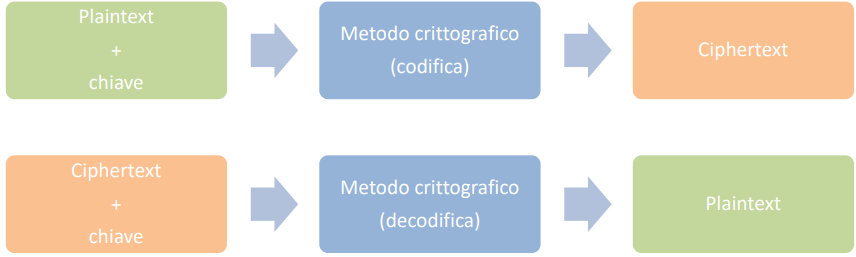
\includegraphics[width=6.26772in,height=3.63889in]{media/image19.png}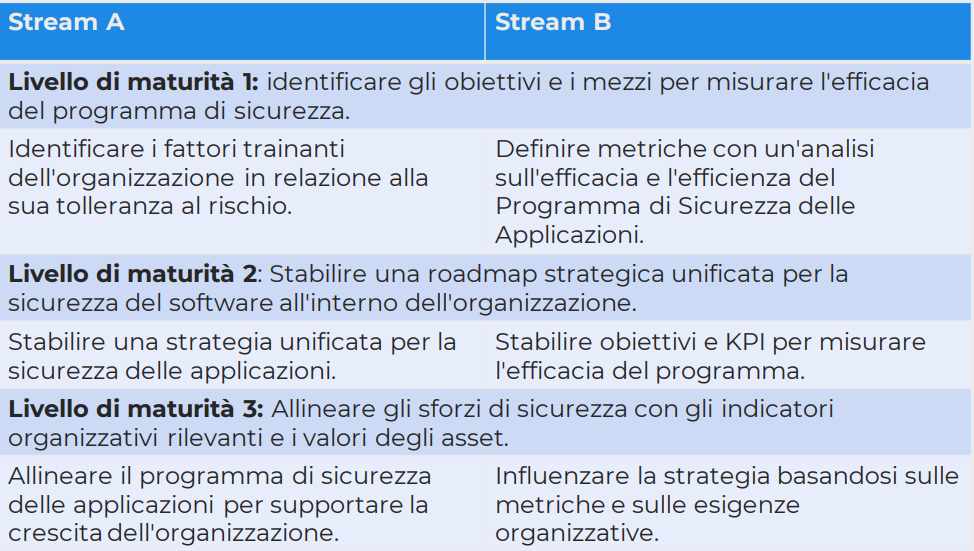
\includegraphics[width=6.26772in,height=2.16667in]{media/image13.png}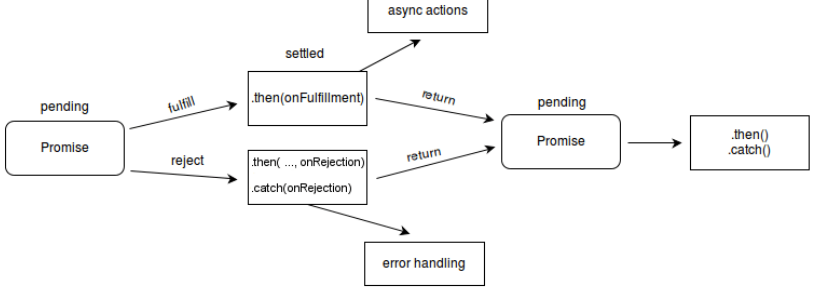
\includegraphics[width=6.26772in,height=2.77778in]{media/image7.png}

\subsection{Domande sbagliate per
orale}\label{domande-sbagliate-per-orale}

\begin{enumerate}
\def\labelenumi{\arabic{enumi}.}
\item
  Cosa viene eseguito al riavvio di un device Arduino? Un bootloader.
\item
  Nelle organizzazioni di task concorrenti\ldots{} ogni task è descritto
  tramite una singola macchina a stati finiti.
\item
  Le porte che permettono la gestione dei pin I/O\ldots{} sono gestiti
  da uno o più registri special purpose.
\item
  Nei dispositivi IoT non aventi un clock interno ma connessi a
  internet, cosa posso utilizzare per ottenere l'orario corretto? Si usa
  un server NTP che però è esterno e non dentro il router, se fosse
  dentro il router anche senza internet avremmo avuto l'orario corretto.
\item
  Quale fra queste NON è un'attività dei S.O? Gestione della
  comunicazione tra programmi.
\item
  Nel protocollo LoraWAN un messaggio di downlink può sempre essere
  inviato in quale di queste casistiche? In nessuna, i messaggi downlink
  vengono inviati solo come risposta di uno uplink non importa la
  classe.
\item
  Il duty cicle nel protocollo LoraWan\ldots{} NON è inversamente
  proporzionale alla dimensione dei pacchetti, ma è il massimo tempo di
  trasmissione per un determinato periodo di tempo.
\item
  Quando una variabile condivisa da task deve essere in sezione critica
  per garantire il corretto funzionamento? Solo se i task sono in
  scrittura, se è in lettura invece non c'è bisogno.
\item
  Se ho un sensore di temperatura collegato alla corrente elettrica, in
  grado di comunicare ad intervalli di 30 minuti \emph{con un requisito
  funzionale di una temperatura media ogni 5 minuti (ogni 5 minuti
  voglio il valore medio di temperatura di quel periodo)} campionamento
  ogni 500ms quale tempo utilizzo per ogni step della macchina a stati?
  Un secondo.
\item
  Quale tra le seguenti caratteristiche è legate a errori accidentali?
  La precisione.
\item
  Per gestire la comunicazione in modo asincrono\ldots{} si possono
  utilizzare code di messaggi.
\item
  Quali delle seguenti affermazioni su UART è falsa? L'UART utilizza una
  comunicazione sincrona. Infatti è asincrono, si appoggia a dispositivi
  separati per gestire i flussi di dati e utilizza un bus seriale.
\item
  I gateway LoraWAN\ldots{} sono l'unico accesso alla rete internet.
\end{enumerate}
